%===============================================================================

\documentclass[conference]{IEEEtran}
% Include all packages from file.
% Report template for Mälardalen University
% Original template can be found: 
% https://www.overleaf.com/latex/templates/ieee-bare-demo-template-for-conferences/ypypvwjmvtdf
% Template file structure organised by: Emil Persson
% The following packages should follow the IEEE conference guidelines.

%===============================================================================
% QoL

%===============================================================================
% Add packages here

\usepackage{comment}
\usepackage[nolist,nohyperlinks]{acronym}
\usepackage{datetime}
\usepackage{amsmath}
\usepackage{cuted}
\usepackage{pdfpages}

% Tables
\usepackage{tabularx}
\usepackage{longtable}
\usepackage[table,xcdraw]{xcolor}

%===============================================================================
%===============================================================================
% Define accronyms here

% Universities
\acrodef{udea}[UdeA]{Universidad de Antioquia}
\acrodef{utp}[UTP]{Universidad Tecnológica de Panamá}
\acrodef{mdu}[MDU]{Mälardalens Universitet}

% Management
\acrodef{wbs}[WBS]{Work Breakdown Structure}
\acrodef{bom}[BOM]{Bill of Materials}

% Software
\acrodef{ai}[AI]{Artificial Intelligence}
\acrodef{api}[API]{Application Programming Interface}
\acrodef{ros2}[ROS2]{Robot Operating System 2}
\acrodef{hil}[HIL]{Hardware-in-the-Loop}
\acrodef{mappo}[MAPPO]{Multi-Agent Proximal Policy Optimization}
\acrodef{udp}[UDP]{User Datagram Protocol}
\acrodef{ppo}[PPO]{Proximal Policy Optimization}
\acrodef{foc}[FOC]{Field-Oriented Control}
\acrodef{ros}[ROS]{Robot Operating System}
\acrodef{gui}[GUI]{Graphical user interface}

% Hardware
\acrodef{cad}[CAD]{Computer-aided Design}
\acrodef{ic}[IC]{Integrated Circuit}
\acrodef{imu}[IMU]{Inertial Measurement Unit}
\acrodef{pcb}[PCB]{Printed Circuit Board}
\acrodef{mcu}[MCU]{Micro Controller Unit}
\acrodef{lidar}[LIDAR]{Light Detection and Ranging}
\acrodef{cpu}[CPU]{Central Processing Unit}
\acrodef{spi}[SPI]{Serial Peripheral Interface}
\acrodef{esc}[ESC]{Electronic Speed Controller}
\acrodef{i2c}[I$^2$C]{Inter-Integrated Circuit}
\acrodef{uart}[UART]{Universal Asynchronous Receiver-Transmitter}
\acrodef{pc}[PC]{Personal Computer}
\acrodef{gpio}[GPIO]{General-Purpose Input/Output}
\acrodef{pwm}[PWM]{Pulse-Width Modulation}

% SSL
\acrodef{ssl}[SSL]{Small Size League}

% Physics

%===============================================================================
%===============================================================================
% Do definitions here

\definecolor{na}{RGB}{130, 130, 130} % Gray for N/A

\definecolor{c}{RGB}{255, 100, 100} % Red for Canceled

\definecolor{h}{RGB}{255, 255, 0} % Yellow for On Hold

\definecolor{p}{RGB}{255, 165, 0} % Orange for progress

\definecolor{d}{RGB}{90, 255, 90}  % Green for completed (done)

\definecolor{u}{RGB}{180, 180, 255} % Blue for upcoming

%===============================================================================

%===============================================================================
% Template stuff

% Swedish language package 
\usepackage[utf8]{inputenc}
\usepackage[T1]{fontenc}
\usepackage[swedish,english]{babel}

% Graphics
\usepackage{graphicx, float, subfigure, blindtext}

\newcommand\IEEEhyperrefsetup{
bookmarks=true,bookmarksnumbered=true,%
colorlinks=true,linkcolor={black},citecolor={black},urlcolor={black}%
}

% Preferred hyperref setup, Michael Shell
\usepackage[\IEEEhyperrefsetup, pdftex]{hyperref}

% Maths
\usepackage{mathtools}

% These packages must be at the end
\usepackage{cleveref}
\graphicspath{{images/}}

% Remove section first paragraph indent
\usepackage{titlesec}
\titlespacing*{\section}{0pt}{*1}{*1}
\titlespacing*{\subsection}{0pt}{*1}{*1}
\renewcommand{\thesubsubsection}{\arabic{subsubsection}}
\titleformat{\subsubsection}[runin]{\itshape}{\thesubsubsection)}{1em}{}[:]
\titlespacing*{\subsubsection}{\parindent}{0pt}{*1}

%===============================================================================
% Authors

% Include authors 
\author{\IEEEauthorblockN{ %
Viktor Eriksson\IEEEauthorrefmark{1},
Anton Grusell\IEEEauthorrefmark{2}, 
Mudar Ibrahim\IEEEauthorrefmark{3},
Jacob Johanssson\IEEEauthorrefmark{4},
Aaiza Aziz Khan\IEEEauthorrefmark{5},
Carl Larsson\IEEEauthorrefmark{6},\\
Johanna Melander\IEEEauthorrefmark{7},
Shruti Puthiya Kunnon\IEEEauthorrefmark{8},
Pontus Svensson\IEEEauthorrefmark{9},
Fredrik Westerbom\IEEEauthorrefmark{10},
Emil Åberg\IEEEauthorrefmark{11}
}
\IEEEauthorblockA{
School of Innovation, Design and Engineering, M.Sc.Eng Robotics\\
Mälardalens University, Västerås, Sweden\\
Email:
\{\IEEEauthorrefmark{1}Ven20002, 
\IEEEauthorrefmark{2}agl19003,
\IEEEauthorrefmark{3}mim20004,
\IEEEauthorrefmark{4}jjn20030,
\IEEEauthorrefmark{5}akn23018,
\IEEEauthorrefmark{6}cln20001,\\
\IEEEauthorrefmark{7}Jmr19002,
\IEEEauthorrefmark{8}spn23001,
\IEEEauthorrefmark{9}psn19003,
\IEEEauthorrefmark{10}fnl18001, 
\IEEEauthorrefmark{11}eag24002\}@student.mdu.se
}}

%===============================================================================
% Title

% The report title.
\title{Multi-robot Soccer - RoboCup - PRO2\\
Mälardalen University}
% Document begins here
\begin{document}

%===============================================================================
% Commands needs to be included here for commands to work in document

%===============================================================================
% Define commands here

% dd-mm-yyyy format
% with zero padding to two digits for month and day
\makeatletter
\renewcommand{\today}{\the\year-\two@digits{\the\month}-\two@digits{\the\day}}
\makeatother

%===============================================================================

%===============================================================================
% Header stuff

% Create the title.
\maketitle
% Create date
\begin{strip}
    \begin{center}
        \today
    \end{center}
\end{strip}

%===============================================================================
% Sections

% Example sections, name them
% according to specific needs.
%===============================================================================
\section{Project Information}

% Project name
This paper covers the progress report for the project Multi-robot Soccer - RoboCup for the time period from 7th of October to 8th of November. 
% Collaboration
This is a collaboration project between \ac{mdu}, \ac{udea} and \ac{utp}. 
% Summary of project 
The project is about creating a \ac{ssl}-RoboCup robot and developing the accompanying software.
It is assumed the reader is familiar with the project, for those who are not, see the project plan available in Appendix\:\ref{appendix}.
% Project members, their roles and their tasks
Table.\:\ref{tab:contributors_roles} outlines the team members, their roles and their assigned tasks.
\begin{table}[H]
    \centering
    \begin{tabularx}{\columnwidth}{|X|X|X|} \hline
         \textbf{Name}          & \textbf{Role}                                         & \textbf{Task}                                 \\ \hline
         Viktor Eriksson        & Software developer                                    & Collective robot behaviour                    \\ \hline
         Anton Grusell          & Hardware developer                                    & 3D-\acs{cad} \& Body design                   \\ \hline
         Mudar Ibrahim          & Team leader \& Software developer                     & Communication                                 \\ \hline
         Jacob Johanssson       & Software developer                                    & Collective robot behaviour                    \\ \hline
         Aaiza Aziz Khan        & Software developer                                    & Communication                                 \\ \hline
         Carl Larsson           & Software lead \& Software developer                   & Individual robot behaviour                    \\ \hline
         Johanna Melander       & Hardware developer                                    & Mechanical design                             \\ \hline
         Shruthi Puthiya Kunnon & Software developer                                    & Communication                                 \\ \hline
         Pontus Svensson        & Team leader \& Hardware lead \& Hardware developer    & Power-train \& Electronics                    \\ \hline
         Fredrik Westerbom      & Hardware developer \& Software developer              & Sensors \& Hardware communication             \\ \hline
         Emil Åberg             & Software developer                                    & Individual robot behaviour \& Communication   \\ \hline
    \end{tabularx}
    \caption{Project contributors, including their roles and assigned tasks.}
    \label{tab:contributors_roles}
\end{table}

%===============================================================================
%===============================================================================
\section{Project Progress Summary}

% !!! Reference back to the project plan !!!

% Provides a concise and informative summary of what has been achieved so far.
% Provide a high-level overview of the project's current status. Briefly mention problematic or delayed work packages, issues, or blockers that require stakeholder attention.


% TEAM LEADER will write this section!! No one is allowed to write here. 


% Overview of work package status 
The project has seen significant progress since it was launched. As of \today,\: 3 out of 14 work packages have been completed, 8 are in progress, 1 has not started yet (upcoming), 2 is on hold and 0 have been cancelled. Note that this does not include the two \ac{hil} work packages which are outside of both the current and the next work period.
% Issues
The projects main threat is time, the project might be able to deliver the individual parts, but the integration of all the parts into a complete functioning package is unrealistic. Additionally, to keep within the limited timeline and budget, optimal and tailor-made solutions had to be sacrificed in favour of simpler ones. This in turn makes it improbable for the final product to function according to the initial demands placed by the stakeholders (capable of competing).
% Stakeholder attention
% Software
The software side of the project is progressing well except for 1.5.5 \textit{nav2 stack configuration} which has proven especially problematic, this still remains to be solved. This has in turn resulted in 1.5.6 \textit{Develop supporting functions} being placed on hold.
% Hardware
The hardware development is progressing but not at the necessary speed to deliver the product by December. Problems with 2.2.1 \textit{Manufacture \acs{pcb}} and the fact that the components have yet to arrive has caused noticeable issues for the hardware team.
See Table.\:\ref{tab:activity_status} for a complete overview of the project status.

%-------------------------------------------------------------------------------

\begin{comment}
Work packages that have been completed are: 
Work packages that are in progress are: 
Work packages that are not started yet are: 

The main issues we had so far are................These issues have caused \textbf{(Delay, blocking or risk of ON track work packages)}
The issues are (solved, still have them) and we plan to solve them by...... 
\end{comment}

%===============================================================================
%===============================================================================
\section{Work Package Status}

% !!! Reference back to the project plan !!!

% !!! ONLY WORK PACKAGES SHOULD BE COVERED !!!

All information regarding the work packages which are apart of the 7th of October to 8th of November work period are covered in the following subsections. Note that only work packages are covered.
%-----------------------------------------------
% Description of columns:

% ID: ID of task/workpackage/deliverable.

% Name: Name of task/workpackage/deliverable.

% Planning status: "On-track" or "Off-track".

% Completion status:  "Not started", "On Hold", "Cancelled", "In Progress", or "Completed".

% Accountability: People responsible for the package.

% Recovery plan: If a package is "Off-track" then here you write the plan to get it back "On-track".

% Progress: Summary of progress, highlighting key outcomes and which tasks/deliverables have been completed. Include both ID and name of tasks and deliverables.

% Issues: List challenges/issues.

% Next steps: Outline the work package's next set of tasks or milestones. List the next deliverables and task which will be done, their ID and name.
%-----------------------------------------------

%-------------------------------------------------------------------------------

\subsection*{1.1 Simulate 12 robots}
\begin{itemize}
    \item \textbf{Planning status}: On-track
    \item \textbf{Completion status}: Completed
    \item \textbf{Accountability}: Aaiza Aziz Khan, Shruthi Puthiya Kunnon, Emil Åberg
    \item \textbf{Recovery plan}: N/A
    \item \textbf{Progress}: Completed all the deliverables and tasks.
    \item \textbf{Issues}: N/A
    \item \textbf{Next steps}: N/A
\end{itemize}

%-------------------------------------------------------------------------------

\subsection*{1.1.2 Simulation interface}
\begin{itemize}
    \item \textbf{Planning status}: On-track
    \item \textbf{Completion status}: Completed
    \item \textbf{Accountability}: Aaiza Aziz Khan, Shruthi Puthiya Kunnon, Emil Åberg
    \item \textbf{Recovery plan}: N/A
    \item \textbf{Progress}: Completed all the deliverables and tasks.
    \item \textbf{Issues}: grSim crashed suddenly and remained in an unusable state until it was fixed by following the troubleshooting instructions in the \href{https://github.com/RoboCup-SSL/grSim/blob/master/INSTALL.md}{INSTALL.md file} available in the \href{https://github.com/RoboCup-SSL/grSim}{grSim repository}. Additionally, a way to control simulation has still not been developed.
    \item \textbf{Next steps}: N/A
\end{itemize}

%-------------------------------------------------------------------------------

\subsection*{1.2 \acs{ssl} interface}
\begin{itemize}
    \item \textbf{Planning status}: On-track
    \item \textbf{Completion status}: Completed
    \item \textbf{Accountability}: Aaiza Aziz Khan, Shruthi Puthiya Kunnon, Emil Åberg
    \item \textbf{Recovery plan}: N/A
    \item \textbf{Progress}: Completed all the deliverables and tasks.
    \item \textbf{Issues}: There are some limitations in how well the clients for ssl-vision and ssl-game-controller can be tested automatically and independently with Google Test; they rely on \ac{udp} streams which need to be generated while the clients are executing in parallel. Therefore, testing of \textit{\acs{ssl} interface} has been complemented with manual tests, where \textit{\acs{ssl} interface} is integrated with ssl-vision and ssl-game-controller.
    \item \textbf{Next steps}: N/A
\end{itemize}

%-------------------------------------------------------------------------------

\subsection*{1.3 Hardware interface}
\begin{itemize}
    \item \textbf{Planning status}: On-Track
    \item \textbf{Completion status}: In Progress
    \item \textbf{Accountability}: Mudar Ibrahim, Aaiza Aziz Khan, Shruthi Puthiya Kunnon, Fredrik Westerbom, Emil Åberg
    \item \textbf{Recovery plan}: N/A
    \item \textbf{Progress}: Currently working on 1.3.5 \textit{Sensor interface}, specifically 1.3.5.1 \textit{\acs{imu}}. 
    \item \textbf{Issues}: Need admin access for installation of STM32CubeIDE to be able to write code for the STM32 board.
    \item \textbf{Next steps}: Sub-work package 1.3.5 \textit{Sensor interface}. 
\end{itemize}

%-------------------------------------------------------------------------------

\subsection*{1.3.5 Sensor interface}
\begin{itemize}
    \item \textbf{Planning status}: On-Track
    \item \textbf{Completion status}: In Progress
    \item \textbf{Accountability}: Mudar Ibrahim, Aaiza Aziz Khan, Shruthi Puthiya Kunnon, Fredrik Westerbom, Emil Åberg
    \item \textbf{Recovery plan}: N/A
    \item \textbf{Progress}: Deliverable 1.3.5.1 \textit{\acs{imu}} is ongoing however, implementation of \ac{spi} has been cancelled due to the support of \ac{i2c} for the \acs{imu}, \ac{lidar}, and RGB sensor. 
    \item \textbf{Issues}: Unforeseen issues understanding and implementing the skeleton code generated by the graphical programming environment. Therefore the implementation of code has been delayed.
    \item \textbf{Next steps}: 1.3.5.1.2. \textit{\acs{i2c} implementation}, 1.3.5.1.3. \textit{\acs{uart} implementation}. Then the rest of the Deliverables 1.3.5.2 - 1.3.5.6
\end{itemize}

%-------------------------------------------------------------------------------

\subsection*{1.4 Communication protocol}
\begin{itemize}
    \item \textbf{Planning status}: On-Track
    \item \textbf{Completion status}: On Hold
    \item \textbf{Accountability}: Aaiza Aziz Khan, Shruthi Puthiya Kunnon, Emil Åberg
    \item \textbf{Recovery plan}: N/A
    \item \textbf{Progress}: Work has begun on establishing communication between PC and Raspberry Pi (1.4.1).   
    \item \textbf{Issues}: HDMI is not available.
    \item \textbf{Next steps}: Ability to send and receive data.
\end{itemize}

%-------------------------------------------------------------------------------
\subsection*{1.5 Individual robot behaviour}
\begin{itemize}
    \item \textbf{Planning status}: Off-track
    \item \textbf{Completion status}: In Progress
    \item \textbf{Accountability}: Carl Larsson
    \item \textbf{Recovery plan}: Enlist additional resources internally (Pontus Svensson, the only other experianced nav2 and \ac{ros2} developer) and enlist external resources (post the problem on Stack Exchange).
    \item \textbf{Progress}: All other deliverables and tasks except 1.5.5 \textit{nav2 stack configuration} and the sub-work package 1.5.6 \textit{Develop supporting functions} have been completed. 1.5.5 \textit{nav2 stack configuration} is currently being worked on.
    \item \textbf{Issues}: Creating proper unit and integration tests for more advanced and interwoven parts of the code. 1.5.5 \textit{nav2 stack configuration} is proving problematic and has taken significantly longer time to complete than expected, this has caused 1.5.6 to be placed On Hold.
    \item \textbf{Next steps}: 1.5.6 \textit{Develop supporting functions}.
\end{itemize}

%-------------------------------------------------------------------------------

\subsection*{1.5.6 Develop supporting functions}
\begin{itemize}
    \item \textbf{Planning status}: On-track
    \item \textbf{Completion status}: On Hold
    \item \textbf{Accountability}: Carl Larsson
    \item \textbf{Recovery plan}: N/A
    \item \textbf{Progress}: Work has started on 1.5.6.1 \textit{Run Simulation/Hardware interface}, specifically integrating the \textit{Simulation interface} (1.5.6.1.1), no noteworthy progress has been made thus far.
    \item \textbf{Issues}: Waiting for 1.4 \textit{Communication protocol} to be completed before being able to start working on 1.5.6.2 \textit{Ability to send data}, \textit{1.5.6.3 Ability to receive data}, \textit{1.5.6.4 Initialize the robot}.
    \item \textbf{Next steps}: 1.5.6.2 \textit{Ability to send data}, 1.5.6.3 \textit{Ability to receive data}, 1.5.6.4 \textit{Initialize the robot}.
\end{itemize}

%-------------------------------------------------------------------------------

\subsection*{1.6 Collective robot behaviour}
\begin{itemize}
    \item \textbf{Planning status}: On-Track
    \item \textbf{Completion status}: In Progress
    \item \textbf{Accountability}: Viktor Eriksson, Jacob Johansson
    \item \textbf{Recovery plan}: N/A
    \item \textbf{Progress}: Completed 1.6.1 \textit{Research \acs{ai}-algorithms}. Working on task 1.6.2.1 \textit{Develop the \acs{ai}-algorithm}, finishing the structure for the \ac{mappo} algorithm. 1.6.4 is currently in progress and will result in the ability to receive data from the external systems.
    \item \textbf{Issues}: Lack of documentation on libraries (i.e. PyTorch) has slowed down the development of the algorithm and functions.
    \item \textbf{Next steps}: 1.6.3 \textit{Be able to send data}.
\end{itemize}

%-------------------------------------------------------------------------------

\subsection*{2.1 Base design}
\begin{itemize}
    \item \textbf{Planning status}: On-Track
    \item \textbf{Completion status}: In Progress
    \item \textbf{Accountability}: Anton Grusell, Johanna Melander, Pontus Svensson, Fredrik Westerbom
    \item \textbf{Recovery plan}: N/A
    \item \textbf{Progress}: 2.1.1 \textit{Hardware design to meet \acs{ssl}-rules} and 2.1.2 \textit{Design modular components} completed. 2.1.3 \textit{3D-design} and 2.1.4 \textit{Circuit design and integration} is in progress.
    \item \textbf{Issues}: Components went out of stock. Restrictions on which components could be used due to collaboration with \ac{udea}.
    \item \textbf{Next steps}: 2.1.3 \textit{3D-design}, 2.1.4 \textit{Circuit design and integration}.
\end{itemize}

%-------------------------------------------------------------------------------

\subsection*{2.1.3 3D-design}
\begin{itemize}
    \item \textbf{Planning status}: On-Track
    \item \textbf{Completion status}: In Progress
    \item \textbf{Accountability}: Anton Grusell, Johanna Melander, Pontus Svensson, Fredrik Westerbom
    \item \textbf{Recovery plan}: N/A
    \item \textbf{Progress}: 2.1.3.1 \textit{Chassis design} waiting for completion of the circuits before continuing. 2.1.3.2 \textit{Wheels design} is in the final stages, awaiting feedback from the manufacturer. 2.1.3.3, 2.1.3.4 and 2.1.3.5 are all in progress. 
    \item \textbf{Issues}: Size requirements makes every decision take more time. As more components are finished, revisions need to be made to ensure compatibility.
    \item \textbf{Next steps}: Finish 2.1.3.3, 2.1.3.4, 2.1.3.5.
\end{itemize}

%-------------------------------------------------------------------------------

\subsection*{2.1.4 Circuit design and integration}
\begin{itemize}
    \item \textbf{Planning status}: On-Track
    \item \textbf{Completion status}: In Progress
    \item \textbf{Accountability}: Anton Grusell, Johanna Melander, Pontus Svensson, Fredrik Westerbom
    \item \textbf{Recovery plan}: If certain circuits are not completed in a timely manner, those functionalities will be excluded from the robot.
    \item \textbf{Progress}: 2.1.4.1 \textit{Design powertrain circuit} is completed. 2.1.4.2 \textit{Design kicker circuit} is completed. 2.1.4.3 \textit{Design dribbler circuit} is completed. 2.1.4.4 \textit{Design microcontroller circuit} is mostly completed, awaiting which type of connector is to be used for mainboard to kicker board connection. 2.1.4.5 \textit{Design \acs{ic} for sensors} is completed. 2.1.4.5.3 \textit{Design break beam \acs{ic}} was cancelled. 2.1.4.6 \textit{Integrate the circuits} is in progress, the pins for the kicker control needs to be decided before the deliverable is completed. 2.1.4.7 \textit{Design mainboard \acs{pcb}} is in progress, dependent on 2.1.4.6. 2.1.4.8 \textit{Design carrier \acs{pcb} for motor driver} is completed. 2.1.4.9 \textit{Design kicker \acs{pcb}} is in progress. 2.1.4.10 \textit{Design basestation \acs{pcb}} was cancelled due to time limitations.
    \item \textbf{Issues}: Finding suitable board-to-board connectors is difficult and expensive, leading to a less suitable option being chosen.
    \item \textbf{Next steps}: 2.2.1 \textit{Manufacture \acs{pcb}}.
\end{itemize}

%===============================================================================

\begin{comment}
\onecolumn
\begin{longtable}{|c|m{0.09\textwidth}|m{0.07\textwidth}|m{0.095\textwidth}|m{0.115\textwidth}|m{0.12\textwidth}|m{0.085\textwidth}|m{0.09\textwidth}|m{0.085\textwidth}|} \hline
\centering
    \textbf{ID} & \textbf{Name} & \textbf{Planning status} & \textbf{Completion status} & \textbf{Accountability} & \textbf{Recovery plan} & \textbf{Progress} & \textbf{Issues} & \textbf{Next steps} \\ \hline
    %---------------------------------------
    % Communication
    %---------------------------------------
    1.1.1 & Setup grSim & On track & Completed & Emil, Aaiza, Shruthi & If anything goes wrong, settings can be restored from grSim Repository & Completed & No issues yet & N/A \\ \hline
    1.1.2.1 & Integrate Protobuf & On track & Completed & Emil, Aaiza, Shruthi & N/A & Completed & No issues yet & N/A \\ \hline
    1.1.2.2 & Move a single robot & On track & Completed & Emil, Aaiza, Shruthi & N/A & Completed & No issues yet & Unit test \\ \hline
    1.1.2.3 & Activate kicker on a single robot & On track & Completed & Emil, Aaiza, Shruthi & N/A & Completed & No issue yet & Unit test \\ \hline
    1.1.2.4 & Execute any desired control over any chosen robot in grSim & On track & Completed & Emil, Aaiza, Shruthi & N/A & Completed & No issue yet & Unit test \\ \hline
    1.2.1 & Integrate ssl-vision & On track & Completed & Emil, Aaiza, Shruthi & N/A & Completed & No issue yet & N/A \\ \hline
    1.2.2 & Integrate ssl-game-controller (human referee and optional auto referee & On track & Completed & Emil, Aaiza, Shruthi & N/A & Completed & No issue yet & Unit tests \\ \hline
    1.2.3 & Develop an automatic game controller (will be used when training the AI) & On track & In progress & Emil, Aaiza, Shruthi & N/A & Unknown & No issues yet & implement own timer \\ \hline
    1.3.1 & Wheel motor interface & On track & Not started & Not decided yet & N/A & 0\% & None & N/A \\ \hline
    1.3.2 & Kicker interface & On track & Not started & Not decided yet & N/A & 0\% & None & N/A \\ \hline
    1.3.3 & Dribbler interface & On track & Not started & Not decided yet & N/A & 0\% & None & N/A \\ \hline
    1.3.4 & Sensor interface & On track & Not started & Not decided yet & N/A & 0\% & None & N/A \\ \hline
    1.4.1 & Integrate Protobuf for Communication Protocol & On track & Not started & Emil, Aaiza, Shruthi & N/A & 0\% & None & N/A \\ \hline
    1.4.2 & Utilize ROS2 for Communication Protocol & On track & Not started yet & Emil, Aaiza, Shruthi & N/A & 0\% & None & N/A \\ \hline
    1.4.3 & Ability to switch between two carrier frequencies & On track & Not started yet & Emil, Aaiza, Shruthi & N/A & 0\% & None & N/A \\ \hline
    %---------------------------------------
    % Individual robot behaviour
    %---------------------------------------
    1.5.1 & Research viable path planning algorithms & On-track & Completed & Carl Larsson & N/A & Completed & No issues encountered & N/A \\ \hline
    1.5.2 & Integrate ROS2 & On-track & Completed & Carl Larsson & N/A & Completed & Uncertainty of how to interact with Hardware Interface & N/A \\ \hline
    1.5.3 & Develop path planning algorithm & On-track & Completed & Carl Larsson & N/A & Completed & Difficult to unit test since it is dependent on the entire nav2 stack & N/A \\ \hline
    1.5.4 & Implement robot ability to shoot & On-track & Completed & Carl Larsson & N/A & Completed & Difficult to unit test since it is dependent on other parts of the system & N/A \\ \hline
    1.5.5.1 & Initialize the robot & On-track & Not started & Carl Larsson & N/A & No tasks completed, awaiting communication protocol completion & No issues encountered yet & Next task 1.5.5.1.1 \\ \hline
    1.5.5.2 & Ability to send data & On-track & Not started & Carl Larsson & N/A & No tasks completed, awaiting communication protocol completion & No issues encountered yet & Next task 1.5.5.2.1 \\ \hline
    1.5.5.3 & Ability to receive data & On-track & Not started & Carl Larsson & N/A & No tasks completed, awaiting communication protocol completion & No issues encountered yet & Next task 1.5.5.3.1 \\ \hline
    %---------------------------------------
    % Collective robot behaviour
    %---------------------------------------
    1.7 & Collective robot behaviour & On track & in progress & Jacob, Viktor & N/A & Finishing the structure of the MAPPO algorithm, some missing functions is needed and communication to the grSim for training & Lack of documentation (MAPPO, pytorch, previous competitors) & Simulate in the real environment. \\ \hline
    1.7.1 & Using Artificial Intelligence for strategy planning & On track & Not started & Jacob, Viktor & Recover the saved model with best result & No finished model yet, thus the reinforced learning will be used to gain strategy planning & No issues encountered yet & Train the AI-algorithm \\ \hline
    1.7.1.1 & Research for the AI-algorithms & Done & Completed & Jacob, Viktor & N/A & Completed & Lack of documentation (MAPPO, pytorch, previous competitors) & Develop the AI-algorithm\\ \hline
    1.7.1.2 & Develop the AI-algorithm & On track & In progress & Jacob, Viktor & Upload all files to Git & 60\% & Lacking information of the C++ pytorch api & Merge to ssl-interface to run in grSim \\ \hline
    1.7.1.3 & Train the AI-algorithm & On track & Not started & Jacob, Viktor & N/A & 0\% & N/A & Develop into hardware \\ \hline
    
    %---------------------------------------
    % Hardware
    %---------------------------------------
    2.1.1 & Hardware design to meet SSL-rules & On track & Done &  Anton, Pontus, Fredik, Johanna & N/A & Completed & N/A & N/A \\ \hline
    2.1.2 & Design modular components & On track & Done &  Anton, Pontus & N/A & Completed & N/A & N/A \\ \hline
    2.1.3 & 3D-Design & On track & In progress & Anton & N/A & 70\% & Final \ac{pcb} are not manufactured yet & Waiting for the \ac{pcb} to be manufactured\\ \hline
    %2.1.2.1 & Chassi design & TEXT & in progress & Anton & unknown & 70\% & No issues yet & waiting for the circuit board designs. \\ \hline
    %2.1.2.2 & Wheels design & On track & Completed & Anton, Johanna & unknown & Completed & No issues yet & Have the parts manufactured. \\ \hline
    2.1.4.1 & Design powertrain circuit & Late & in progrss & Pontus & N/A & 90\% & Due to delay in approval of components the workpackage has been delayed & Finish the circuit\\ \hline
    2.1.4.2 & Design kicker circuit & On track & Completed & Johanna & N/A & Completed & N/A & N/A\\ \hline
    %2.1.3.1 & Design Powertrain & TEXT & TEXT &  & TEXT & TEXT & TEXT & TEXT \\ \hline
    %2.1.3.2 & Design Kicker & Late & In progress & Johanna & TEXT & 70\% & Switched a key component, so the circuit needs to be updated & Update the circuit \\ \hline
    2.1.4.3 & Design Dribbler & Late & In progress & Anton & N/A & 80\% & More difficult to design in a way that makes it fit than initially thought. &  N/A \\ \hline
    2.1.4.4 & Design microcontroller circuit & Late & In progress & Pontus & N/A & 70\% & Due to delay in choosing \ac{mcu} the circuit is not completed & Complete the circuit\\ \hline
    2.1.4.5 & Design \ac{ic} for sensors & On track & Completed & Fredrik & N/A & Completed & None & N/A \\ \hline
    % 2.1.4.1 & Design encoder \ac{ic} & On track & Completed & Fredrik & N/A & Completed & None & Unit test (task 2.2.1.6) \\ \hline
    % 2.1.4.2 & Design Break Beam \ac{ic} & On track & Completed & Fredrik & N/A & Completed & None & Unit test (task 2.2.1.5) \\ \hline
    % 2.1.4.3 & Design \ac{imu} \ac{ic} & On track & Completed & Fredrik & N/A & Completed & None & Unit test (task 2.2.1.4 \\ \hline    
    2.1.4.6 & Integrate the circuits & Late & In progress & Pontus & N/A & 50\% & Waiting on 2.1.4.1 and 2.1.4.4 & Finish the dependent tasks \\ \hline
    2.1.4.7 & Design mainboard \ac{pcb} & Late & In progress & Pontus & N/A & 30\% & N/A & Finish dependent workpackages. \\ \hline
    2.1.4.8 & Design carrier \ac{pcb} for motor driver & On track & In progress & Pontus & A design was received from Delft Mercurians SSL team. & 90\% & N/A & N/A \\ \hline
    2.1.4.9 & Design kicker PCB & On track & Not started & Johanna & N/A & 0\%& N/A &\\ \hline
    2.1.4.10 & Design basestation \ac{pcb} & On track & In progress & Pontus & Basestation is based on Tiger Mannheim & Completed & Some components are difficult to source & Manufacture the \ac{pcb}. \\ \hline 
    2.2.1 & Manufacture \ac{pcb} & On track & Not started & Pontus & If no sponsor is found, PCBway will be used to manufacture. & 0\% & Difficulties finding a sponsor. & Find a sponsor. \\ \hline
    2.3.1 & Test motors & On track & Not started & Pontus & N/A & 0\% & N/A & N/A \\ \hline
    2.3.2 & Test kicker & On track & Not started & Johanna & N/A & 0\% & N/A & N/A \\ \hline
    2.3.3 & Test Dribbler & On track & Not started & Anton & N/A & 0\% & N/A & N/A \\ \hline
    2.3.4 & Test sensors & On track & Not started & Fredrik & N/A & 0\% & N/A & N/A \\ \hline
    2.3.5 & Validate the integrated circuits & On track & Not started & Fredrik, Pontus, Anton, Johanna & N/A & 0\% & N/A & N/A \\ \hline
    2.4.1 & Basestation communication & On track & Not started & Fredrik & N/A & 0\% & N/A & N/A \\ \hline
    2.4.2 & Motor driver interface & On track & Not started & Pontus & N/A & 0\% & N/A & N/A \\ \hline
    2.4.3 & Kicker interface & On track & Not started & Johanna & N/A & 0\% & N/A & N/A \\ \hline
    2.4.4 & Develop Dribbler interface & On track & Not started & Anton & N/A & 0\% & N/A & N/A \\ \hline
    
    \caption{The status of each work package which is part of the time period from 7th of October to 8th of November.}
    \label{tab:work_package_status}
\end{longtable}
\twocolumn
\end{comment}

%===============================================================================
%===============================================================================
\section{Completed and Upcoming Activities}

% Milestones achieved
The project has achieved the following milestones thus far:
\begin{itemize}
    \item \textit{Simulation interface} done
    \item \textit{SSL interface} done
\end{itemize}
% Completed and Upcoming Activities
The completed and the upcoming activities for the project are shown in Table.\:\ref{tab:activity_status}, which is the \ac{wbs} with the addition of a new column indicating the status of the activity. Note that any activity which is outside of the next work period, spanning from November 8 to December 6, is seen as N/A (-).

\onecolumn
\begin{longtable}{|c|c|m{0.6\textwidth}|c|} \hline
    \centering
%-------------------------------------------------------------------------------
    \textbf{ID} & \textbf{Work Class} & \textbf{Name (Work entailed)} & \textbf{Status} \\ \hline
    \rowcolor{na} - & Root & Multi-robot Soccer - RoboCup & - \\ \hline
    %--------------------
    % Software
    %--------------------
    \rowcolor{p} 1 & Category & Software & In Progress \\ \hline
    \rowcolor{d} 1.1 & Work Package & Simulate 12 robots & Completed \\ \hline
    \rowcolor{d} 1.1.1 & Deliverable & Setup grSim & Completed \\ \hline
    \rowcolor{d} 1.1.1.1 & Task & Download grSim & Completed \\ \hline
    \rowcolor{d} 1.1.1.2 & Task & Run the simulation correctly & Completed \\ \hline
    \rowcolor{d} 1.1.2 & Work Package & Simulation interface (\acs{api}) & Completed \\ \hline
    \rowcolor{d} 1.1.2.1 & Deliverable & Integrate Protobuf & Completed \\ \hline
    \rowcolor{d} 1.1.2.2 & Deliverable & Move a single robot & Completed \\ \hline
    \rowcolor{d} 1.1.2.3 & Deliverable & Activate kicker on a single robot & Completed \\ \hline
    \rowcolor{d} 1.1.2.4 & Deliverable & Activate dribbler on a single robot & Completed \\ \hline
    \rowcolor{d} 1.1.2.5 & Deliverable & Execute any desired control over any chosen robot in grSim & Completed \\ \hline
    \rowcolor{d} 1.2 & Work Package & \acs{ssl} interface (\acs{api}) & Completed \\ \hline
    \rowcolor{d} 1.2.1 & Deliverable & Integrate ssl-vision & Completed \\ \hline
    \rowcolor{d} 1.2.1.1 & Task & Receive single package containing positional data & Completed \\ \hline
    \rowcolor{d} 1.2.1.2 & Task & Receive continuous positional data & Completed \\ \hline
    \rowcolor{d} 1.2.2 & Deliverable & Integrate ssl-game-controller (human referee and optional auto referee) & Completed \\ \hline
    \rowcolor{d} 1.2.2.1 & Task & Receive a single package containing referee commands/signals & Completed \\ \hline
    \rowcolor{d} 1.2.2.2 & Task & Receive continuous stream of referee commands/signals & Completed \\ \hline
    \rowcolor{d} 1.2.2.3 & Task & Integrate AutoReferee & Completed \\ \hline
    \rowcolor{d} 1.2.3 & Deliverable & Develop an automatic game controller (will be used when training the \acs{ai}) & Completed \\ \hline
    \rowcolor{d} 1.2.3.1 & Task & Research and obtain proper understanding of \acs{ssl}-rules & Completed \\ \hline
    \rowcolor{d} 1.2.3.2 & Task & Implement the automatic game controller system & Completed \\ \hline
    \rowcolor{p} 1.3 & Work Package & Hardware interface (\acs{api}) & In Progress \\ \hline
    \rowcolor{c} 1.3.1 & Deliverable & Basestation communication & Cancelled \\ \hline
    \rowcolor{c} 1.3.1.1 & Task & Configure basestation RF communication & Cancelled \\ \hline
    \rowcolor{p} 1.3.2 & Deliverable & Wheel motor interface & In Progress \\ \hline
    \rowcolor{p} 1.3.2.1 & Task & Establish communication using \acs{uart} & In Progress \\ \hline
    \rowcolor{u} 1.3.2.2 & Task & Implement \acs{foc} & Upcoming \\ \hline
    \rowcolor{u} 1.3.2.3 & Task & Implement a velocity distributor (subscribing to cmd\_vel) & Upcoming \\ \hline
    \rowcolor{u} 1.3.3 & Deliverable & Kicker interface & Upcoming \\ \hline
    \rowcolor{u} 1.3.3.1 & Task & \acs{gpio} implement activation & Upcoming \\ \hline
    \rowcolor{u} 1.3.4 & Deliverable & Dribbler interface & Upcoming \\ \hline
    \rowcolor{u} 1.3.4.1 & Task & Implement \acs{pwm} control & Upcoming \\ \hline
    \rowcolor{p} 1.3.5 & Work Package & Sensor interface & In Progress \\ \hline
    \rowcolor{p} 1.3.5.1 & Deliverable & \acs{imu} & In Progress \\ \hline
    \rowcolor{c} 1.3.5.1.1 & Task & \acs{spi} implementation & Cancelled \\ \hline
    \rowcolor{p} 1.3.5.1.2 & Task & \acs{i2c} implementation & In Progress \\ \hline
    \rowcolor{u} 1.3.5.1.3 & Task & Communicate using \acs{uart} & Upcoming \\ \hline
    \rowcolor{u} 1.3.5.2 & Deliverable & Wheel encoders & Upcoming \\ \hline
    \rowcolor{u} 1.3.5.2.1 & Task & Configure wheel encoders & Upcoming \\ \hline
    \rowcolor{u} 1.3.5.3 & Deliverable & Camera & Upcoming \\ \hline
    \rowcolor{u} 1.3.5.4 & Deliverable & \acs{lidar} & Upcoming \\ \hline
    \rowcolor{u} 1.3.5.4.1 & Task & \acs{i2c} implementation & Upcoming \\ \hline
    \rowcolor{u} 1.3.5.4.2 & Task & Communicate using \acs{uart} & Upcoming \\ \hline
    \rowcolor{u} 1.3.5.5 & Deliverable & RGB sensor & Upcoming \\ \hline
    \rowcolor{u} 1.3.5.5.1 & Task & \acs{i2c} implementation & Upcoming \\ \hline
    \rowcolor{u} 1.3.5.5.2 & Task & Communicate using \acs{uart} & Upcoming \\ \hline
    \rowcolor{u} 1.3.5.6 & Deliverable & Break beam & Upcoming \\ \hline
    \rowcolor{u} 1.3.6 & Deliverable & Provide robot status information & Upcoming \\ \hline
    \rowcolor{u} 1.3.6.1 & Task & \acs{cpu} temperature & Upcoming \\ \hline
    \rowcolor{u} 1.3.6.2 & Task & Battery charge & Upcoming \\ \hline
    \rowcolor{p} 1.3.7 & Deliverable & Establish communication between Raspberry Pi and Nucleo 144 & In Progress \\ \hline
    \rowcolor{p} 1.3.7.2 & Task & Install micro-\acs{ros} on Raspberry Pi and Nucleo 144 (\acs{uart}) & In Progress \\ \hline
    \rowcolor{u} 1.3.7.3 & Task & Implement \acs{ros} functionality & Upcoming \\ \hline
    \rowcolor{u} 1.3.8 & Deliverable & Establish communication between Nucleo 144 and motor drivers & Upcoming \\ \hline
    \rowcolor{u} 1.3.8.1 & Task & Communicating using \acs{uart} & Upcoming \\ \hline
    \rowcolor{h} 1.4 & Work Package & Communication protocol (\acs{api}) & On Hold \\ \hline
    \rowcolor{h} 1.4.1 & Deliverable & Establish communication between \acs{pc} and Raspberry Pi & On Hold \\ \hline
    \rowcolor{h} 1.4.1.1 & Task & Using Wi-Fi & On Hold \\ \hline
    \rowcolor{u} 1.4.2 & Deliverable & Integrate Protobuf & Upcoming \\ \hline
    \rowcolor{u} 1.4.3 & Deliverable & Utilizing \acs{ros2} & Upcoming \\ \hline
    \rowcolor{u} 1.4.4 & Deliverable & Ability to switch between two carrier frequencies & Upcoming \\ \hline
    \rowcolor{p} 1.5 & Work Package & Individual robot behaviour (finding the best way to do the things it has been commanded to do) & In Progress \\ \hline
    \rowcolor{d} 1.5.1 & Deliverable & Research viable path planning algorithms & Completed \\ \hline
    \rowcolor{d} 1.5.2 & Deliverable & Integrate \acs{ros2} & Completed \\ \hline
    \rowcolor{d} 1.5.2.1 & Task & Getting sensor data & Completed \\ \hline
    \rowcolor{d} 1.5.2.2 & Task & Getting odometry data & Completed \\ \hline
    \rowcolor{d} 1.5.3 & Deliverable & Develop path planning algorithm & Completed \\ \hline
    \rowcolor{d} 1.5.3.1 & Task & Build using nav2 & Completed \\ \hline
    \rowcolor{d} 1.5.4 & Deliverable & Implement robot ability to shoot & Completed \\ \hline
    \rowcolor{d} 1.5.4.1 & Task & Angle correctly towards target & Completed \\ \hline
    \rowcolor{d} 1.5.4.2 & Task & Shoot towards target & Completed \\ \hline
    \rowcolor{p} 1.5.5 & Deliverable & nav2 stack configuration & In Progress \\ \hline
    \rowcolor{p} 1.5.5.1 & Task & Create nav2 parameter files & In Progress \\ \hline
    \rowcolor{p} 1.5.5.2 & Task & Create nav2 launch files & In Progress \\ \hline
    \rowcolor{h} 1.5.6 & Work Package & Develop supporting functions & On Hold \\ \hline
    \rowcolor{h} 1.5.6.1 & Deliverable & Run Simulation/Hardware interface & On Hold \\ \hline
    \rowcolor{h} 1.5.6.1.1 & Task & Run and call on Simulation interface & On Hold \\ \hline
    \rowcolor{h} 1.5.6.1.2 & Task & Run and call on Hardware interface & On Hold \\ \hline
    \rowcolor{h} 1.5.6.2 & Deliverable & Ability to send data & On Hold \\ \hline
    \rowcolor{h} 1.5.6.2.1 & Task & Sending robot status (\acs{cpu} temperature and battery charge) & On Hold \\ \hline
    \rowcolor{h} 1.5.6.2.2 & Task & Sending acknowledgements that commanded task has been completed & On Hold \\ \hline
    \rowcolor{h} 1.5.6.3 & Deliverable & Ability to receive data & On Hold \\ \hline
    \rowcolor{h} 1.5.6.3.1 & Task & Ability to receive initialization data from collective robot behaviour (ID, home playing side, starting pose) & On Hold \\ \hline
    \rowcolor{h}1.5.6.3.2 & Task & Ability to receive control commands from collective robot behaviour & On Hold \\ \hline
    \rowcolor{h} 1.5.6.3.3 & Task & Ability to receive pose correction data from collective robot behaviour & On Hold \\ \hline
    \rowcolor{h} 1.5.6.4 & Deliverable & Initialize the robot & On Hold \\ \hline
    \rowcolor{h} 1.5.6.4.1 & Task & Getting robot ID & On Hold \\ \hline
    \rowcolor{h} 1.5.6.4.2 & Task & Obtaining information about which playing side of the field is friendly & On Hold \\ \hline
    \rowcolor{h} 1.5.6.4.3 & Task & Getting the start pose & On Hold \\ \hline
    \rowcolor{p} 1.6 & Work Package & Collective robot behaviour/ Centralised strategy planner (Handles what each individual robot should do to obtain a win for the team) & In Progress \\ \hline
    \rowcolor{d} 1.6.1 & Deliverable & Research \acs{ai}-algorithms & Completed \\ \hline
    \rowcolor{d} 1.6.1.1 & Task & Outline actions & Completed \\ \hline
    \rowcolor{d} 1.6.1.2 & Task & Outline world representation (input) & Completed \\ \hline
    \rowcolor{p} 1.6.2 & Deliverable & Develop \acs{ai} for strategy planning & In Progress \\ \hline
    \rowcolor{p} 1.6.2.1 & Task & Develop the \acs{ai}-algorithm & In Progress \\ \hline
    \rowcolor{u} 1.6.2.2 & Task & Train the \acs{ai}-algorithm & Upcoming \\ \hline
    \rowcolor{u} 1.6.3 & Deliverable & Be able to send data & Upcoming \\ \hline
    \rowcolor{u} 1.6.3.1 & Task & Provide initialization data to all robots & Upcoming \\ \hline
    \rowcolor{u} 1.6.3.2 & Task & Be able to send control commands to robots & Upcoming \\ \hline
    \rowcolor{u} 1.6.3.3 & Task & Be able to send pose correction data to robots & Upcoming \\ \hline
    \rowcolor{p} 1.6.4 & Deliverable & Be able to receive data & In Progress \\ \hline
    \rowcolor{p} 1.6.4.1 & Task & Be able to receive robot status information & In Progress \\ \hline
    \rowcolor{p} 1.6.4.2 & Task & Be able to receive referee commands and signals from \acs{ssl} interface & In Progress \\ \hline
    \rowcolor{d} 1.6.4.3 & Task & Be able to receive positional data from \acs{ssl} interface & Completed \\ \hline
    \rowcolor{u} 1.6.5 & Deliverable & Ability to switch playing half on demand & Upcoming \\ \hline
    %--------------------
    % Hardware
    %--------------------
    \rowcolor{p} 2 & Category & Hardware & In Progress \\ \hline
    \rowcolor{p} 2.1 & Work Package & Base design & In Progress \\ \hline
    \rowcolor{d} 2.1.1 & Deliverable & Hardware design to meet \acs{ssl}-rules & Completed \\ \hline
    \rowcolor{d} 2.1.1.1 & Task & Research for chassis design & Completed \\ \hline
    \rowcolor{d} 2.1.1.2 & Task & Chassis \acs{bom} & Completed \\ \hline
    \rowcolor{d} 2.1.1.3 & Task & Powertrain \acs{bom} & Completed \\ \hline
    \rowcolor{d} 2.1.1.4 & Task & Sensor \acs{bom} & Completed \\ \hline
    \rowcolor{d} 2.1.1.5 & Task & Kicker \acs{bom} & Completed \\ \hline
    \rowcolor{d} 2.1.2 & Deliverable & Design modular components & Completed \\ \hline
    \rowcolor{d} 2.1.2.1 & Task & Allow for battery swap & Completed \\ \hline
    \rowcolor{d} 2.1.2.2 & Task & Allow for motor swap & Completed \\ \hline
    \rowcolor{p} 2.1.3 & Work Package & 3D-design & In Progress \\ \hline
    \rowcolor{d} 2.1.3.1 & Deliverable & Chassis design & Completed \\ \hline
    \rowcolor{d} 2.1.3.2 & Deliverable & Wheel design & Completed \\ \hline
    \rowcolor{d} 2.1.3.2.1 & Task & Wheel hub design & Completed \\ \hline
    \rowcolor{d} 2.1.3.2.1 & Task & Subwheel design & Completed \\ \hline
    \rowcolor{p} 2.1.3.3 & Deliverable & Dribbler design & In Progress \\ \hline
    \rowcolor{d} 2.1.3.4 & Deliverable & Kicker assembly design & Completed \\ \hline
    \rowcolor{p} 2.1.3.5 & Deliverable & Mounting design & In Progress \\ \hline
    \rowcolor{p} 2.1.3.5.1 & Task & Encoder mount & In Progress \\ \hline
    \rowcolor{d} 2.1.3.5.2 & Task & Motor mount & Completed \\ \hline
    \rowcolor{d} 2.1.3.5.3 & Task & Battery mount & Completed \\ \hline
    \rowcolor{d} 2.1.3.5.4 & Task & Dribbler mount & Completed \\ \hline
    \rowcolor{p} 2.1.4 & Work Package & Circuit design and integration & In Progress \\ \hline
    \rowcolor{d} 2.1.4.1 & Deliverable & Design powertrain circuit & Completed \\ \hline
    \rowcolor{p} 2.1.4.2 & Deliverable & Design kicker circuit & In Progress \\ \hline
    \rowcolor{d} 2.1.4.3 & Deliverable & Design dribbler circuit & Completed \\ \hline
    \rowcolor{d} 2.1.4.4 & Deliverable & Design microcontroller circuit & Completed \\ \hline
    \rowcolor{d} 2.1.4.5 & Deliverable & Design \acs{ic} for sensors & Completed \\ \hline
    \rowcolor{d} 2.1.4.5.1 & Task & Design \acs{imu} \acs{ic} & Completed \\ \hline
    \rowcolor{d} 2.1.4.5.2 & Task & Design wheel encoder \acs{ic} & Completed \\ \hline
    \rowcolor{c} 2.1.4.5.3 & Task & Design break beam \acs{ic} & Cancelled \\ \hline
    \rowcolor{p} 2.1.4.6 & Deliverable & Integrate the circuits & In Progress \\ \hline
    \rowcolor{d} 2.1.4.7 & Deliverable & Design mainboard \acs{pcb} & Completed \\ \hline
    \rowcolor{d} 2.1.4.8 & Deliverable & Design carrier \acs{pcb} for motor driver & Completed \\ \hline
    \rowcolor{p} 2.1.4.9 & Deliverable & Design kicker \acs{pcb} & In Progress \\ \hline
    \rowcolor{c} 2.1.4.10 & Deliverable & Design basestation \acs{pcb} & Cancelled \\ \hline
    \rowcolor{p} 2.2 & Work Package & Manufacturing & In Progress \\ \hline
    \rowcolor{p} 2.2.1 & Deliverable & Manufacture \acs{pcb} & In Progress \\ \hline
    \rowcolor{d} 2.2.1.1 & Task & Mainboard & Completed \\ \hline
    \rowcolor{c} 2.2.1.2 & Task & Basestation & Cancelled \\ \hline
    \rowcolor{u} 2.2.1.3 & Task & Kicker board & Upcoming\\ \hline
    \rowcolor{d} 2.2.1.4 & Task & Motor driver carrier board & Completed \\ \hline
    \rowcolor{u} 2.2.2 & Deliverable & Manufacture 3D-designed items & Upcoming \\ \hline
    \rowcolor{u} 2.2.2.1 & Task & Manufacture chassis & Upcoming \\ \hline
    \rowcolor{u} 2.2.2.2 & Task & Manufacture wheels & Upcoming \\ \hline
    \rowcolor{u} 2.2.2.3 & Task & Manufacture dribbler & Upcoming \\ \hline
    \rowcolor{u} 2.2.2.4 & Task & Manufacture kicker assembly & Upcoming \\ \hline
    \rowcolor{u} 2.2.2.5 & Task & Manufacture mountings & Upcoming \\ \hline
    \rowcolor{u} 2.3 & Work Package & Testing & Upcoming \\ \hline
    \rowcolor{u} 2.3.1 & Deliverable & Test motors & Upcoming \\ \hline
    \rowcolor{u} 2.3.2 & Deliverable & Test kicker & Upcoming \\ \hline
    \rowcolor{u} 2.3.3 & Deliverable & Test dribbler & Upcoming \\ \hline
    \rowcolor{u} 2.3.4 & Deliverable & Test sensors & Upcoming \\ \hline
    \rowcolor{u} 2.3.4.1 & Task & Test \acs{imu} & Upcoming \\ \hline
    \rowcolor{u} 2.3.4.2 & Task & Test wheel encoders & Upcoming \\ \hline
    \rowcolor{u} 2.3.4.3 & Task & Test camera & Upcoming \\ \hline
    \rowcolor{u} 2.3.4.4 & Task & Test \acs{lidar} & Upcoming \\ \hline
    \rowcolor{u} 2.3.4.5 & Task & Test RGB sensor & Upcoming \\ \hline
    \rowcolor{u} 2.3.5 & Deliverable & Validate the integrated circuits & Upcoming \\ \hline
    \rowcolor{u} 2.3.5.1 & Task & Battery works correctly & Upcoming \\ \hline
    \rowcolor{u} 2.3.5.2 & Task & \acs{ssl}-rule compliance & Upcoming \\ \hline
    %--------------------
    % HIL
    %--------------------
    \rowcolor{na} 3 & Category & \acs{hil} & - \\ \hline
    \rowcolor{na} 3.1 & Work Package & Develop \acs{hil} & - \\ \hline
    \rowcolor{na} 3.1.1 & Deliverable & Design a system to integrate hardware in simulation & - \\ \hline
    \rowcolor{na} 3.1.2 & Deliverable & Test the \acs{hil} in simulation & - \\ \hline
    \rowcolor{na} 3.1.3 & Deliverable & Ensure a smooth transition from simulation to physical robot hardware & - \\ \hline
    \rowcolor{na} 3.2 & Work Package & Validate hardware platform & - \\ \hline
    \rowcolor{na} 3.2.1 & Deliverable & Conduct \acs{hil} test to validate the performance & - \\ \hline
%-------------------------------------------------------------------------------
    \caption{Summary of completed and upcoming activities. Green for completed, orange for in progress, yellow for on hold, red for cancelled, blue for upcoming (part of the next work period which spans from November 8 to December 6) and gray for N/A (-). N/A (-) is anything outside the next work period (November 8 to December 6).}
    \label{tab:activity_status}
\end{longtable}
\twocolumn

%===============================================================================
%===============================================================================
\section{Issues, Blockers, and Risks Status}

% !!! Reference back to the project plan !!!

% Identify any issues or blockers that are currently affecting the project.
% Outline the steps being taken to mitigate these concerns.

% Identifies any problems or obstacles hindering the progress and potential risks, along with their resolution or mitigation plans.

A number of issues were identified, and in an attempt to minimise their impact on the project they were combined with a mitigation action. The issues and their corresponding mitigation plan can be seen in Table.\:\ref{tab:issues_and_mitigation}. 
\begin{table}[H]
    \centering
    \begin{tabularx}{\columnwidth}{|X|X|} \hline
         \textbf{Issue} & \textbf{Mitigation} \\ \hline
         1.2 \& 1.6: Compilation error in centralised-ai repository after merge & Allocate additional work force to solve the problem. \\ \hline
         1.5: nav2 stack error & Enlisting Pontus Svenssons help (the only other member with \ac{ros2} and nav2 experience). Additionally, asking the question on Stack Exchange to allow external resources to help find the answer. \\ \hline
         1.3.5: Difficulty implementing \ac{spi} & Reading from multiple sources online, reading manuals and data sheets. Looking at examples provided by Würth. Will look at the examples provided by STMicroelectronics, as well as other competitive teams such as TIGERs Mannheim and Delft Mercurians. \\ \hline
         2.1.3: Size constraints for parts & Redesigning and moving already made \ac{cad} models to make more room to fit components. \\ \hline
         1: Software modules have so far only been tested individually. There may be issues or even necessary functionality that is missing that is only apparent once integration has been attempted. & Integrate different software modules at the earliest possible moment, thus leaving time to fix any potential issues which might arise. \\ \hline
         1.1.2: Simulation is currently limited to only being able to run in real time. Without being able to control speed of simulation, the capacity to train the \ac{ai} model will be significantly reduced. & Dedicate time to try and find a way to control simulation speed. Worst case scenario, the loss of \ac{ai} performance has to be accepted. \\ \hline
         2: Components arriving late, this will delay development and testing of components. & The \textit{Hardware interface} will be implemented until the components arrive. \\ \hline
         2.2: No sponsor for \ac{pcb} manufacturing has been found. & The project will use an external \ac{pcb} supplier. \\ \hline
    \end{tabularx}
    \caption{All identified issues and the steps being taken to mitigate them.}
    \label{tab:issues_and_mitigation}
\end{table}


%===============================================================================
%===============================================================================
\section{Individual Contributions}

% !!! Reference back to the project plan !!!

% Contributions
This section will provide a summary of what each team member has worked on, their challenges and their contributions to the project goals:
%-------------------------------------------------------------------------------
\subsection*{Viktor Eriksson}
\begin{itemize}
    \item \textbf{Work}: Did research on \ac{ai}-algorithms 1.6.1, and then started to develop the \ac{ai} 1.6.2.1. Will be using \acf{mappo} algorithm for centralised strategy planing.
    \item \textbf{Challenges}: The amount of information found about \ac{mappo} was very limited, the most informative paper does not provide fully correct information and contains misspellings. Despite this, \ac{mappo} was chosen because the algorithm has proven to be efficient in multi agent reinforcement learning applications. Additional challenges include combining other team members codes and having to adapt the code to make the integration work.
    \item \textbf{Contributions to project goals}: Develop the strategy planing 1.6.2.
\end{itemize}
%-------------------------------------------------------------------------------
\subsection*{Anton Grusell}
\begin{itemize}
    \item \textbf{Work}: 2.1.1.2 \textit{Chassis \acs{bom}}, 2.1.3 \textit{3D-design}, 2.1.3.1 \textit{Chassis design}, 2.1.3.2 \textit{Wheel design}, 2.1.3.3 \textit{Dribbler design}, 2.1.3.5 \textit{Mounting design} 2.1.4.3 \textit{Design dribbler circuit}, PRO1, PRO2, 
    \item \textbf{Challenges}: Revisions to designs for compatibility, fulfilling the size constraints. The dribbler design proved problematic when trying to reduce size.
    \item \textbf{Contributions to project goals}: Designing the chassis and wheels in \ac{cad}, designing the dribbler system and a test rig for it. Designing encoder mounts for the wheels. 
\end{itemize}
%-------------------------------------------------------------------------------
\subsection*{Mudar Ibrahim}
\begin{itemize}
    \item \textbf{Work}: Mostly worked on team management, Progress Report structure and keeping work packages on-track. Also worked on 1.3 \textit{Hardware interface}, writing \ac{i2c} communication protocol. Additionally, reviewing this document on a continuous basis. 
    \item \textbf{Challenges}: Using only one STM32 board extended the testing time, since the team had to wait for access to the board to test code.
    Additionally, team management sometimes took longer than expected, causing other tasks to be pushed closer to their deadlines.
    \item \textbf{Contributions to project goals}: 1.3 \textit{Hardware interface} and PRO2 structure. 
\end{itemize}
%-------------------------------------------------------------------------------
\subsection*{Jacob Johansson}
\begin{itemize}
    \item \textbf{Work}: 1.6.1 Helped research state-of-the-art algorithms used for cooperative robots. 1.6.2.1 Develop core functions of the \ac{ai} algorithm.
    \item \textbf{Challenges}: Papers lacking the proper citations for the original sources of certain equations used. This complicated development of the \ac{mappo} algorithm since it caused confusion about which equations was to be used.
    \item \textbf{Contributions to project goals}: Writing functions for the \acf{mappo} algorithm, which dictates the strategy behaviour of the robots.
\end{itemize}
%-------------------------------------------------------------------------------
\subsection*{Aaiza Aziz Khan}
\begin{itemize}
    \item \textbf{Work}: 1.1 \textit{Simulate 12 robots}, 1.1.2 \textit{Simulation interface}, 1.2 \textit{\acs{ssl} interface}.
    \item \textbf{Challenges}: Initial difficulties in familiarising with new techniques, standards and tools.
    \item \textbf{Contributions to project goals}: Contributed in developing ssl-vision client, automatic game controller, and some functions in 1.1.2 and 1.2. Writing test suites for ssl-vision client, ssl-game-controller client and \textit{Simulation interface}.
\end{itemize}
%-------------------------------------------------------------------------------
\subsection*{Carl Larsson}
\begin{itemize}
    \item \textbf{Work}: 1.5 \textit{Individual robot behaviour}, 1.5.6 \textit{Develop supporting functions}, PRO1, PRO2, management and support for the team.
    \item \textbf{Challenges}: Time management and designing a suitable software structure so that the different software parts will be able to be integrated properly. nav2 stack error, prolonging the expected development time of 1.5.5 \textit{nav2 stack configuration} significantly.
    \item \textbf{Contributions to project goals}: Writing code for the executable which will run on the robots, it is tasked with finding a suitable way to realize the commands from the centralized strategy planner. Substantial documentation efforts.
\end{itemize}
%-------------------------------------------------------------------------------
\subsection*{Johanna Melander}
\begin{itemize}
    \item \textbf{Work}: 2.1.1.5 \textit{Kicker \acs{bom}}, 2.1.3.2 \textit{Wheel design}, 2.1.4.2 \textit{Design kicker circuit}, PRO1, PRO2.
    \item \textbf{Challenges}:
    The test solenoid did not arrive on time, so it has not been possible to experiment as much as desired. 
    \item \textbf{Contributions to project goals}:
    Researched about the wheels and kicker design. Designing a simple kicker test rig and an initial version of the wheels in \ac{cad}. Designing kicker circuit in KiCAD, created \ac{bom} for kicker circuit. 
\end{itemize}
%-------------------------------------------------------------------------------
\subsection*{Shruthi Puthiya Kunnon}
\begin{itemize}
    \item \textbf{Work}: Work Packages 1.1 \textit{Simulate 12 robots}, 1.1.2 \textit{Simulation interface}, 1.2 \textit{\acs{ssl} interface}. 
    \item \textbf{Challenges}: Initially, struggled to understand the standards and tools.
    \item \textbf{Contributions to project goals}: Worked on the development of 1.1.2 and 1.2. Developed test suites for \textit{Simulation interface}, \textit{\acs{ssl} interface}, ssl-game-controller. 
\end{itemize}
%-------------------------------------------------------------------------------
\subsection*{Pontus Svensson}
\begin{itemize}
    \item \textbf{Work}: 2.1.1.3 \textit{Powertrain \acs{bom}}, 2.1.2 \textit{Design modular components}, 2.1.4 \textit{Circuit design and integration}, 2.2 \textit{Manufacturing}, 2.2.1.4 ordered motor driver carrier board. Trying to make the collaboration work with \ac{udea} and \ac{utp}.
    \item \textbf{Challenges}: Some initial difficulties regarding which components were allowed to be used, delayed the initial work packages. Size constraints in the robot leads to peculiar solutions for fitting all \acp{esc} and sensors resulting in almost every rule imaginable being broken regarding \ac{pcb} design. 
    \item \textbf{Contributions to project goals}: Designing the mainboard, motor carrier, and encoder \ac{pcb}, reaching out to other teams for guidance and feedback.  
\end{itemize}
%-------------------------------------------------------------------------------
\subsection*{Fredrik Westerbom}
\begin{itemize}
    \item \textbf{Work}: Deliverables 1.3.2, and 1.3.5.1, and 2.1.4.5. Tasks 2.1.1.4, and 2.3.4.1.
    \item \textbf{Challenges}: The task 2.3.4.1 requires a communication protocol to receive and transmit data. \ac{spi} was initially chosen (before abandoned) due to its speed and low latency. Additional pre-requisite tasks have been discovered, the duration of the task has therefore increased. These additional tasks include research into \ac{spi}, installing and getting familiarized with the recommended programming environment as well as the development board NUCLEO-H723ZG.
    Deliverable 1.3.2 is in the startup phase which in short includes pre-studies to familiarize with the development environment as well as acquire the necessary level of understanding to implement \ac{foc}.
    \item \textbf{Contributions to project goals}: The deliverables and tasks are identified to be crucial sub-tasks for the success of the project.
\end{itemize}
%-------------------------------------------------------------------------------
\subsection*{Emil Åberg}
\begin{itemize}
    \item \textbf{Work}: Work Packages 1.1, 1.1.2, organize \textit{\acs{ssl} interface} (Work package 1.2), help with deliverables 1.2.1, 1.2.2, implement collision detection and tests for the automatic game controller (1.2.3.2). Just started on \textit{Hardware interface} (1.3).
    \item \textbf{Challenges}: A way to control simulation speed has not been developed yet. For the sake of training the \ac{ai}, it would be best not to be limited to having it run in real time.
    \item \textbf{Contributions to project goals}: Develop \textit{Simulation interface}, structure and help implement \textit{\acs{ssl} interface}.
\end{itemize}
%-------------------------------------------------------------------------------


%===============================================================================

\begin{comment}
\begin{table}[H]
    \centering
    \begin{tabularx}{\columnwidth}{|c|X|X|X|} \hline
         \textbf{Name} & \textbf{Work} & \textbf{Challenges} & \textbf{Contributions to project goals} \\ \hline
         Viktor Eriksson & Collective robot behaviour&Creating the AI-model in C++, lack of information for the API. & Development of the AI model and strategy planning\\ \hline
         Anton Grusell & 2.1.3 3D-design, 2.1.3.1 Chassi design, 2.1.3.2 Wheel design 2.1.4.3 Design dribbler circuit&  & Working on the robot design and ensuring that everything will fit. Designing a dribbler system.\\ \hline
         Mudar Ibrahim & & & \\ \hline
         Jacob Johansson & 1.7.1.1 Researching MAPPO 1.7.1.2 Develop core functions and tests & Lack of documentation on Pytorch library. &  \\ \hline
         Aaiza Aziz Khan & & & \\ \hline
         Carl Larsson & 1.5.2 Integrate ROS2, 1.5.3 Develop path planning algorithm, 1.5.4 Implement robot ability to shoot, PRO1, PRO2, Management & Time management, Design software structure & Writing code for the executable which will run on the robots, it tasked with finding a suitable way to realize the command from the centralized strategy planner \\ \hline
         Johanna Melander & & & \\ \hline
         Shruthi Puthiya Kunnon & & & \\ \hline
         Pontus Svensson & 2.1.1 Hardware design to meet SSL-rules, 2.1.2 Design modular components, PRO1, PRO2 & Time management, planning and have to redo planning takes a lot of time & Reaching out to companies for help with \ac{pcb} manufacturing. Reaching out to other teams for guidance and knowledge.  \\ \hline
         Fredrik Westerbom & & & \\ \hline
         Emil Åberg & & & \\ \hline
    \end{tabularx}
    \caption{The work done by each team member, the challenges they have encountered and their contributions to the project goals.}
    \label{tab:individual_contributions}
\end{table}
\end{comment}

%===============================================================================

% Select the IEEEtran style
\bibliographystyle{IEEEtran}
% Include bibliography file
%\bibliography{IEEEabrv,references}

\clearpage
%===============================================================================
\onecolumn
\appendix
%===============================================================================
% Project plan
\label{appendix}

% Include project plan pdf
\clearpage
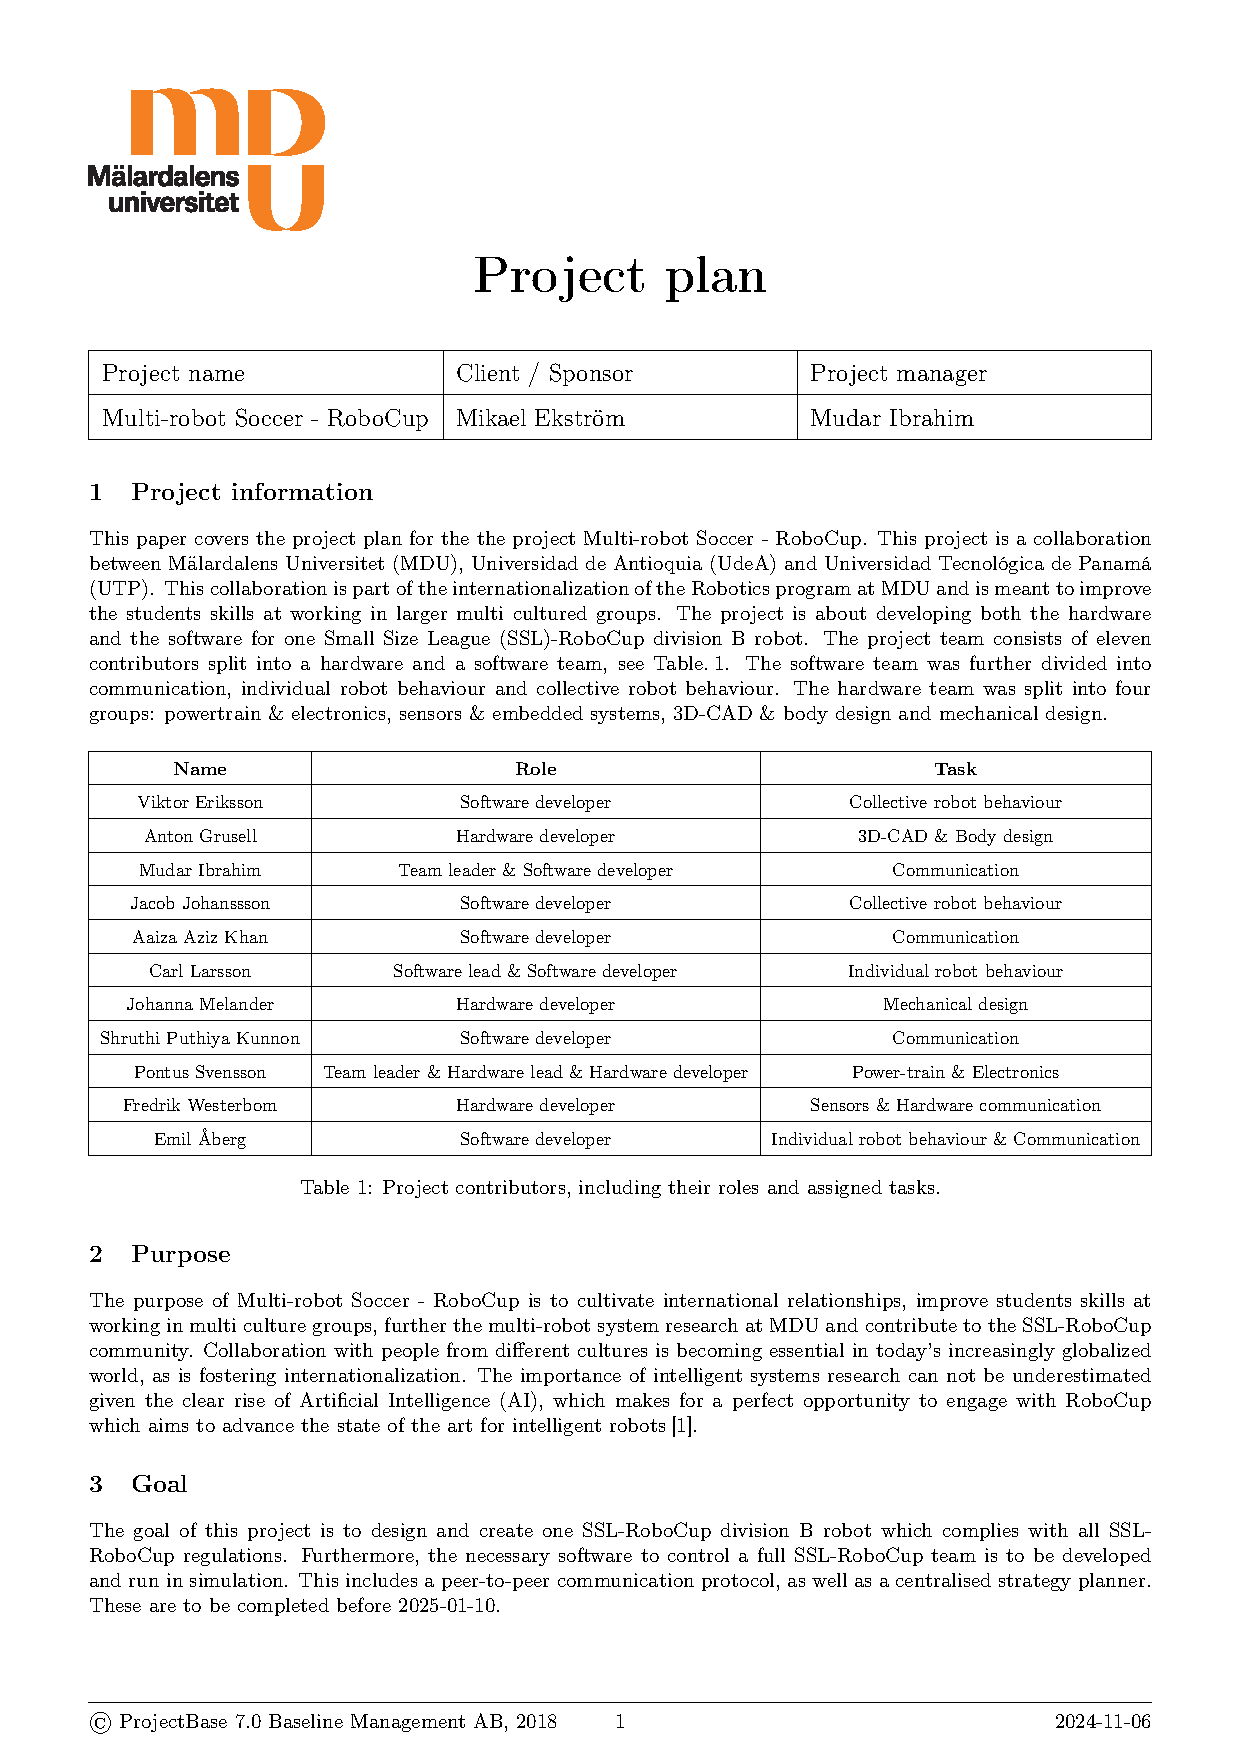
\includepdf[pages={1-}]{files/DVA490_474_PRO1.pdf}

%===============================================================================

%===============================================================================

\end{document}

%===============================================================================